\documentclass[UTF8]{article}
\usepackage{arxiv}
\usepackage{ctex}
\usepackage[utf8]{inputenc} % allow utf-8 input
\usepackage[T1]{fontenc} % use 8-bit T1 fonts
\usepackage{url} % simple URL typesetting
\usepackage{booktabs} % professional-quality tables
\usepackage{amsfonts,amsmath,amssymb} % blackboard math symbols
\usepackage{nicefrac} % compact symbols for 1/2, etc.
\usepackage{microtype} % microtypography
\usepackage{lipsum} % Can be removed after putting your text content
\usepackage{graphicx}
\usepackage{natbib}
\usepackage{doi}
\usepackage{fontspec}
\usepackage{caption}
\usepackage{enumitem}

\usepackage{setspace}
\setlength{\abovecaptionskip}{3pt} % 标题上方间距
\setlength{\belowcaptionskip}{3pt} % 标题下方间距
\setlength{\floatsep}{5pt} % 浮动体（表格/图）与文字的间距

\usepackage{hyperref} % hyperlinks for references
\hypersetup{hidelinks,
colorlinks=true,
linkcolor=red,
citecolor=green
}


\title{
    \textbf{三层神经网络分类器实现与实验分析} \\
    \vspace{8pt}
    \large \textit{深度学习与空间智能课程报告}
}
\author{
    {\hspace{1mm}范鑫宇} \\
    大数据学院\\
    \texttt{25210980034@m.fudan.edu.cn} \\
}


\renewcommand{\headeright}{Report}
\renewcommand{\shorttitle}{深度学习与空间智能课程报告}
\setlength{\parindent}{2em}
\setmainfont{Times New Roman}


\begin{document}
\maketitle

% ============= ABSTRACT ============= %
\begin{abstract}
本文实现了一个从零开始构建的三层神经网络分类器，用于EuroSAT-RGB遥感图像分类任务。该模型不依赖任何深度学习框架，通过NumPy手动实现了神经网络的前向传播、反向传播、激活函数、损失函数和优化器等核心组件。实验结果表明，通过网格搜索超参组合并进行训练后，该模型在EuroSAT测试集上取得了较好的分类性能，测试集准确率达59.83\%，验证了手动实现神经网络的有效性。

\end{abstract}
\keywords{三层神经网络 \and EuroSAT-RGB \and 遥感图像分类 \and 前向传播 \and 反向传播 \and 模型可视化}

\section{引言}
本文通过从零实现一个三层神经网络分类器，探索了神经网络的基本原理和实现细节。

EuroSAT-RGB是一个广泛使用的遥感图像数据集，包含10个类别的卫星图像，是评估遥感图像分类算法性能的标准基准。本项目以EuroSAT-RGB为数据集，实现了一个三层神经网络分类器，通过手动实现核心组件，深入理解神经网络的工作原理。


\section{相关技术基础}

\subsection{神经网络基础}

神经网络通常包含输入层、隐藏层和输出层：

\begin{itemize}[topsep=0pt, partopsep=0pt, itemsep=0pt, parsep=0pt]
    \item 输入层：接收原始数据，对于EuroSAT-RGB图像分类任务，输入层维度为12288（64×64×3）；
    \item 隐藏层：提取数据的特征表示，本文采用两层隐藏层，可自定义大小；
    \item 输出层：产生最终的预测结果，对于EuroSAT-RGB的10个类别，输出层包含10个神经元。
\end{itemize}

神经网络的核心计算包括前向传播和反向传播：

\begin{itemize}[topsep=0pt, partopsep=0pt, itemsep=0pt, parsep=0pt]
    \item 前向传播：数据从输入层流向输出层，计算每一层的输出；
    \item 反向传播：根据预测结果与真实标签的误差，从输出层反向计算梯度，更新网络参数。
\end{itemize}

\subsection{激活函数}

激活函数为神经网络引入非线性。本文实现了多种激活函数，包括Sigmoid、ReLU、Tanh和Softmax，具体汇总如下：

\begin{table}[!htb]
    \centering
    \caption{激活函数汇总}
    \label{tab:activation_functions}
    \begin{tabular}{@{}cccc@{}}
        \toprule
        激活函数 & 数学表达式 & 导数 & 特点 \\
        \midrule
        Sigmoid & $Sigmoid(x) = \frac{1}{1 + e^{-x}}$ & $Sigmoid'(x) = Sigmoid(x) \times (1 - Sigmoid(x))$ & 映射到(0, 1)区间 \\
        ReLU & $ReLU(x) = max(0, x)$ & $ReLU'(x) = \begin{cases} 1, & x > 0 \\ 0, & x \leq 0 \end{cases}$ & 缓解梯度消失问题 \\
        Tanh & $Tanh(x) = tanh(x)$ & $Tanh'(x) = 1 - tanh^2(x)$ & 映射到(-1, 1)区间 \\
        Softmax & $Softmax(x_i) = \frac{e^{x_i}}{\sum_j e^{x_j}}$ & —— & 输出概率分布 \\
        \bottomrule
    \end{tabular}
\end{table}

实验通过超参数搜索比较不同激活函数的性能，最终发现Tanh激活函数在验证集上取得最佳效果。

\subsection{损失函数}

损失函数用于衡量模型预测与真实标签之间的差异。本文使用交叉熵损失函数，适用于多分类问题，公式为：
$$L(y, \hat{y}) = -\sum_{i=1}^{C} y_i \log(\hat{y}_i)$$
其中，$y$是真实标签的one-hot编码，$\hat{y}$是模型的预测概率，$C$是类别数。

\subsection{优化器}

优化器用于更新网络参数。本文使用带动量和L2正则化的随机梯度下降（SGD）优化器，公式为：
$$\nabla L(\theta) = \nabla L_{loss}(\theta) + \lambda \theta$$
$$v_t = \gamma v_{t-1} + \eta \nabla L(\theta)$$
$$\theta = \theta - v_t$$
其中，$v_t$是动量，$\gamma$是动量系数，$\eta$是学习率，$\nabla L_{loss}(\theta)$是损失函数关于参数的梯度，$\lambda$是L2正则化系数。

\subsection{学习率调度}

学习率调度用于在训练过程中调整学习率，本文使用步长衰减（Step Decay）策略，公式为：
$$\eta_t = \eta_0 \times \gamma^{\lfloor t / s \rfloor}$$
其中，$\eta_0$是初始学习率，$\gamma$是衰减因子，$s$是步长，$t$是当前迭代次数。

\section{目标与技术}

\subsection{任务目标}
本项目核心任务是设计并实现一个从零开始构建的三层神经网络分类器，用于EuroSAT-RGB遥感图像分类，具体包括：
\begin{itemize}[topsep=0pt, partopsep=0pt, itemsep=0pt, parsep=0pt]
    \item 自主实现自动微分与反向传播，不依赖任何深度学习框架；
    \item 实现数据加载与预处理、模型定义、训练循环、测试评估、超参数查找五个模块；
    \item 支持自定义隐藏层大小、激活函数切换、学习率衰减和L2正则化；
    \item 进行超参数搜索，优化模型性能；
    \item 可视化训练过程、模型参数和错误分析。
\end{itemize}

\subsection{技术路线}
项目整体技术路线分为以下几个部分：
\begin{itemize}[topsep=0pt, partopsep=0pt, itemsep=0pt, parsep=0pt]
    \item 数据处理：加载EuroSAT-RGB数据集，进行预处理和数据划分；
    \item 模型设计：实现三层神经网络，包括前向传播和反向传播；
    \item 训练优化：实现SGD优化器、学习率衰减和L2正则化；
    \item 超参数搜索：使用网格搜索和随机搜索优化超参数；
    \item 评估分析：评估模型性能，可视化训练过程和模型参数。
\end{itemize}


\section{数据集与模型设计}

\subsection{数据集介绍}

\subsubsection{EuroSAT-RGB数据集}
EuroSAT-RGB是一个基于 Sentinel-2 卫星图像的土地覆盖分类数据集，包含10个类别的遥感图像。每个类别包含不同数量的64×64像素的RGB图像，总计27,000张图像。

\subsubsection{数据集类别}
EuroSAT-RGB数据集包含以下10个类别：
\begin{itemize}[topsep=0pt, partopsep=0pt, itemsep=0pt, parsep=0pt]
    \item AnnualCrop（一年生作物）
    \item Forest（森林）
    \item HerbaceousVegetation（草本植被）
    \item Highway（高速公路）
    \item Industrial（工业区域）
    \item Pasture（牧场）
    \item PermanentCrop（永久作物）
    \item Residential（住宅区）
    \item River（河流）
    \item SeaLake（海洋/湖泊）
\end{itemize}
\subsubsection{数据预处理}
数据预处理步骤包括：
\begin{itemize}[topsep=0pt, partopsep=0pt, itemsep=0pt, parsep=0pt]
    \item 图像加载：使用PIL库加载图像文件；
    \item 尺寸调整：确保所有图像为64×64像素；
    \item 数据标准化：首先将像素值归一化到[0, 1]范围（除以255），然后按通道计算均值和标准差并进行标准化，最后展平数据；
    \item 数据划分：将数据集分为训练集、验证集和测试集，比例为18:2:5。
\end{itemize}
\subsection{模型设计}
\subsubsection{三层神经网络架构}
本文实现的三层神经网络由以下部分组成：
\begin{itemize}[topsep=0pt, partopsep=0pt, itemsep=0pt, parsep=0pt]
    \item 输入层：维度为12288（64×64×3），接收扁平化的图像数据；
    \item 隐藏层1：可自定义大小，使用Tanh激活函数；
    \item 隐藏层2：可自定义大小，使用Tanh激活函数；
    \item 输出层：维度为10，使用Softmax激活函数，输出类别概率分布。
\end{itemize}
\subsubsection{核心组件实现}
\begin{itemize}[topsep=0pt, partopsep=0pt, itemsep=0pt, parsep=0pt]
    \item 激活函数：实现了ReLU、Sigmoid、Tanh等激活函数，支持前向和反向传播；
    \item 损失函数：实现了交叉熵损失函数，支持前向和反向传播；
    \item 优化器：实现了SGD优化器，支持动量和权重衰减；
    \item 学习率调度：实现了步长衰减，指数衰减和ReduceLROnPlateau策略。
\end{itemize}
\subsubsection{模型训练流程}
\begin{enumerate}[topsep=0pt, partopsep=0pt, itemsep=0pt, parsep=0pt]
    \item 初始化模型参数；
    \item 前向传播计算预测值；
    \item 计算损失函数值；
    \item 反向传播计算梯度；
    \item 使用优化器更新参数；
    \item 在验证集上评估模型性能；
    \item 保存性能最佳的模型。
\end{enumerate}
\section{超参数搜索与实验}
\subsection{超参数搜索方法}
\subsubsection{网格搜索}
网格搜索是一种穷举式的超参数优化方法，通过遍历所有可能的超参数组合来寻找最佳配置。本文搜索的超参数包括：
\begin{itemize}[topsep=0pt, partopsep=0pt, itemsep=0pt, parsep=0pt]
    \item 隐藏层大小（hidden-size1, hidden-size2）
    \item 激活函数（hidden-activation）
    \item 学习率（learning-rate）
    \item 动量（momentum）
    \item 权重衰减（weight-decay）
\end{itemize}
\subsubsection{随机搜索}
随机搜索是一种高效的超参数优化方法，通过在超参数空间中随机采样来寻找最佳配置。本文设置了超参数的搜索范围：
\begin{itemize}[topsep=0pt, partopsep=0pt, itemsep=0pt, parsep=0pt]
    \item 隐藏层大小：从预定义列表中随机选择
    \item 学习率：从1e-4到1e-2的对数均匀分布中采样
    \item 动量：从0.8到0.99的均匀分布中采样
    \item 权重衰减：从1e-5到1e-3的对数均匀分布中采样
\end{itemize}
\subsection{实验设置}
\subsubsection{实验环境}
\begin{itemize}[topsep=0pt, partopsep=0pt, itemsep=0pt, parsep=0pt]
    \item 硬件环境：CPU Intel Core i7，GPU NVIDIA GeForce RTX 3060
    \item 软件环境：Python 3.13.0，NumPy 2.0.0
\end{itemize}
\subsection{模型评估指标}
采用准确率（Accuracy）作为模型评估指标，计算公式为：
$$Accuracy = \frac{N_{correct}}{N_{total}}$$
其中，$N_{correct}$ 表示正确分类的样本数，$N_{total}$ 表示总样本数。

同时，使用混淆矩阵（Confusion Matrix）分析模型在各个类别上的表现。

\section{实验结果与分析}
\subsection{超参数搜索结果}
\subsubsection{网格搜索组合情况}
本文进行了网格搜索，训练轮数固定为10，批量大小固定为128。搜索的超参数组合情况如下：
\begin{table}[!htb]
    \centering
    \caption{网格搜索超参数组合及最优配置}
    \label{tab:grid_search_config}
    \begin{tabular}{@{}ccc@{}}
        \toprule
        超参数 & 搜索范围 & 最优组合 \\
        \midrule
        隐藏层1大小 & [128, 256] & 256 \\
        隐藏层2大小 & [64, 128] & 128 \\
        激活函数 & ['relu', 'tanh'] & Tanh \\
        学习率 & [0.1, 0.01] & 0.1 \\
        动量 & [0.0, 0.9] & 0.9 \\
        权重衰减 & [0.0, 0.005, 0.001] & 0.0 \\
        \bottomrule
    \end{tabular}
\end{table}

最佳验证准确率：\textbf{57.27\%}
\subsubsection{超参数组合分析}
本文进行了全面的超参数组合搜索，包括不同的隐藏层大小、激活函数、学习率、动量和权重衰减值。超参数组合的性能分布如图~\ref{fig:hyperparam_combinations}所示：
\begin{figure}[!htb]
    \centering
    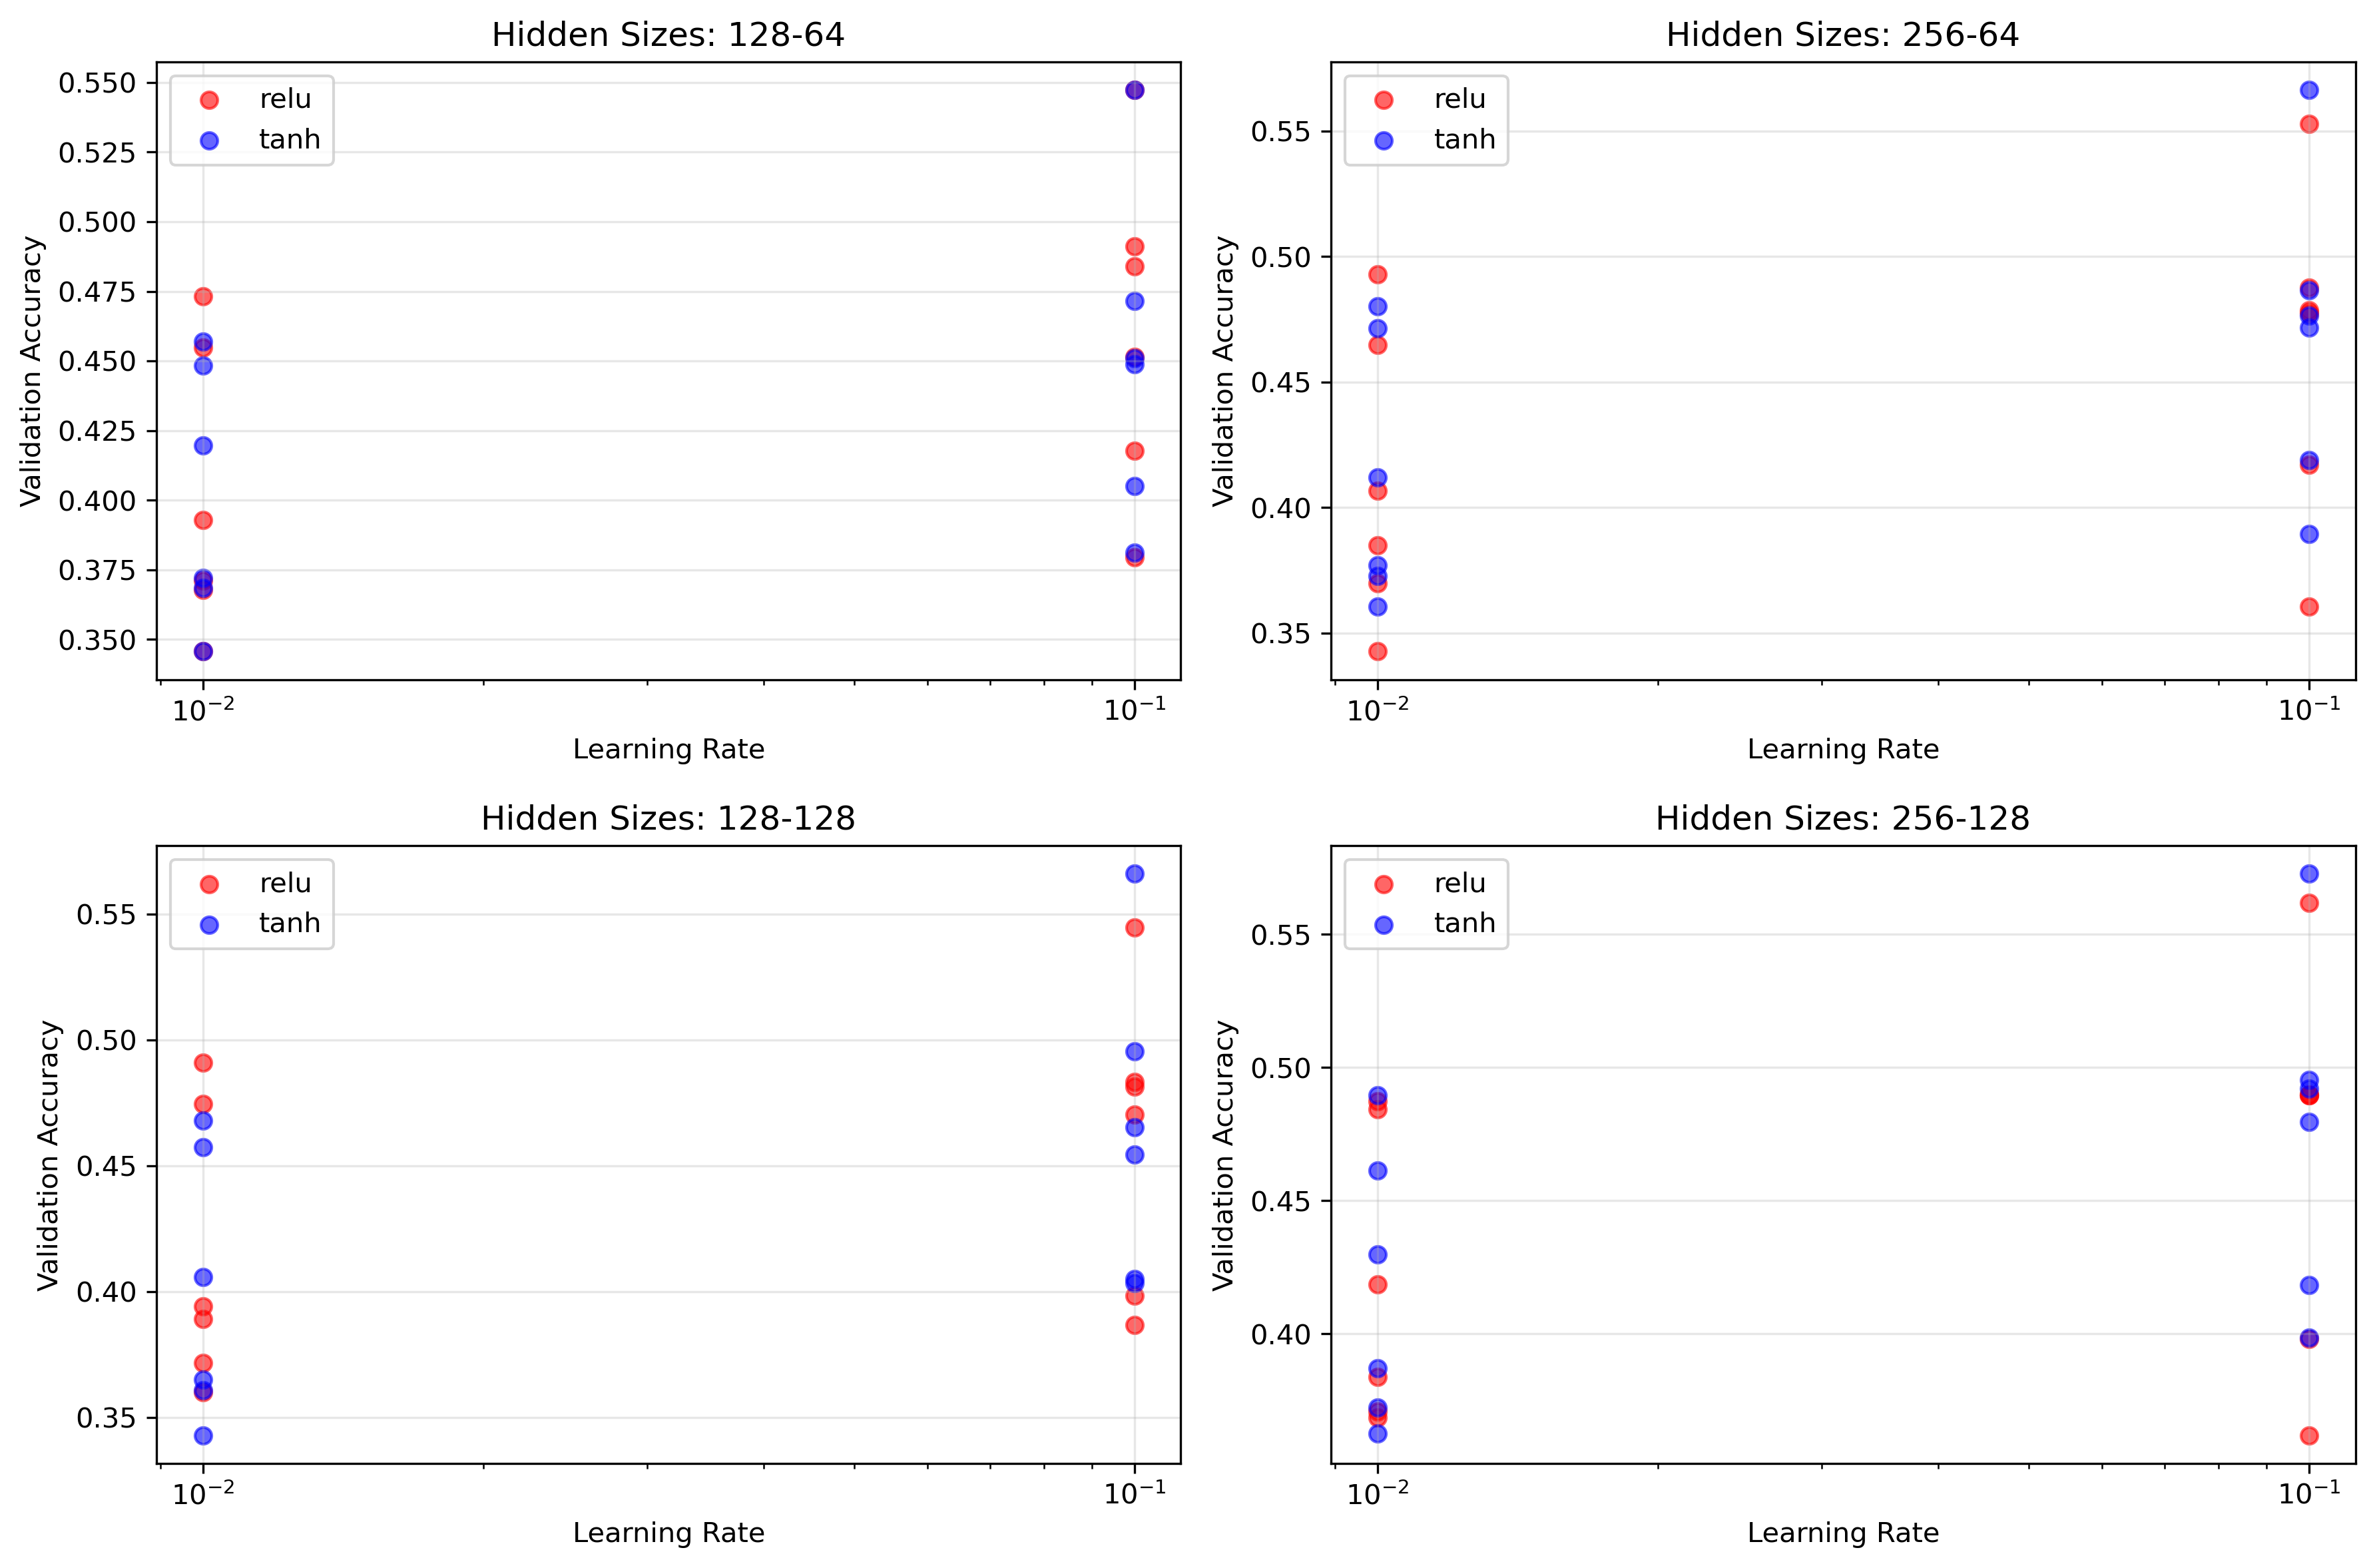
\includegraphics[width=0.9\linewidth]{../search_results/visualizations/hyperparam_combinations.png}
    \captionsetup{font={small,bf}}  % 小号加粗
    \caption{超参数组合与验证准确率的关系}
    \label{fig:hyperparam_combinations}
\end{figure}

从图中可以看出，不同隐藏层大小组合下，学习率和激活函数对模型性能的影响。总体而言，较大的学习率（0.1）和Tanh激活函数能够获得更好的性能。

\subsubsection{超参数重要性分析}
超参数对模型性能的影响程度如图~\ref{fig:hyperparam_importance}所示：
\begin{figure}[!htb]
    \centering
    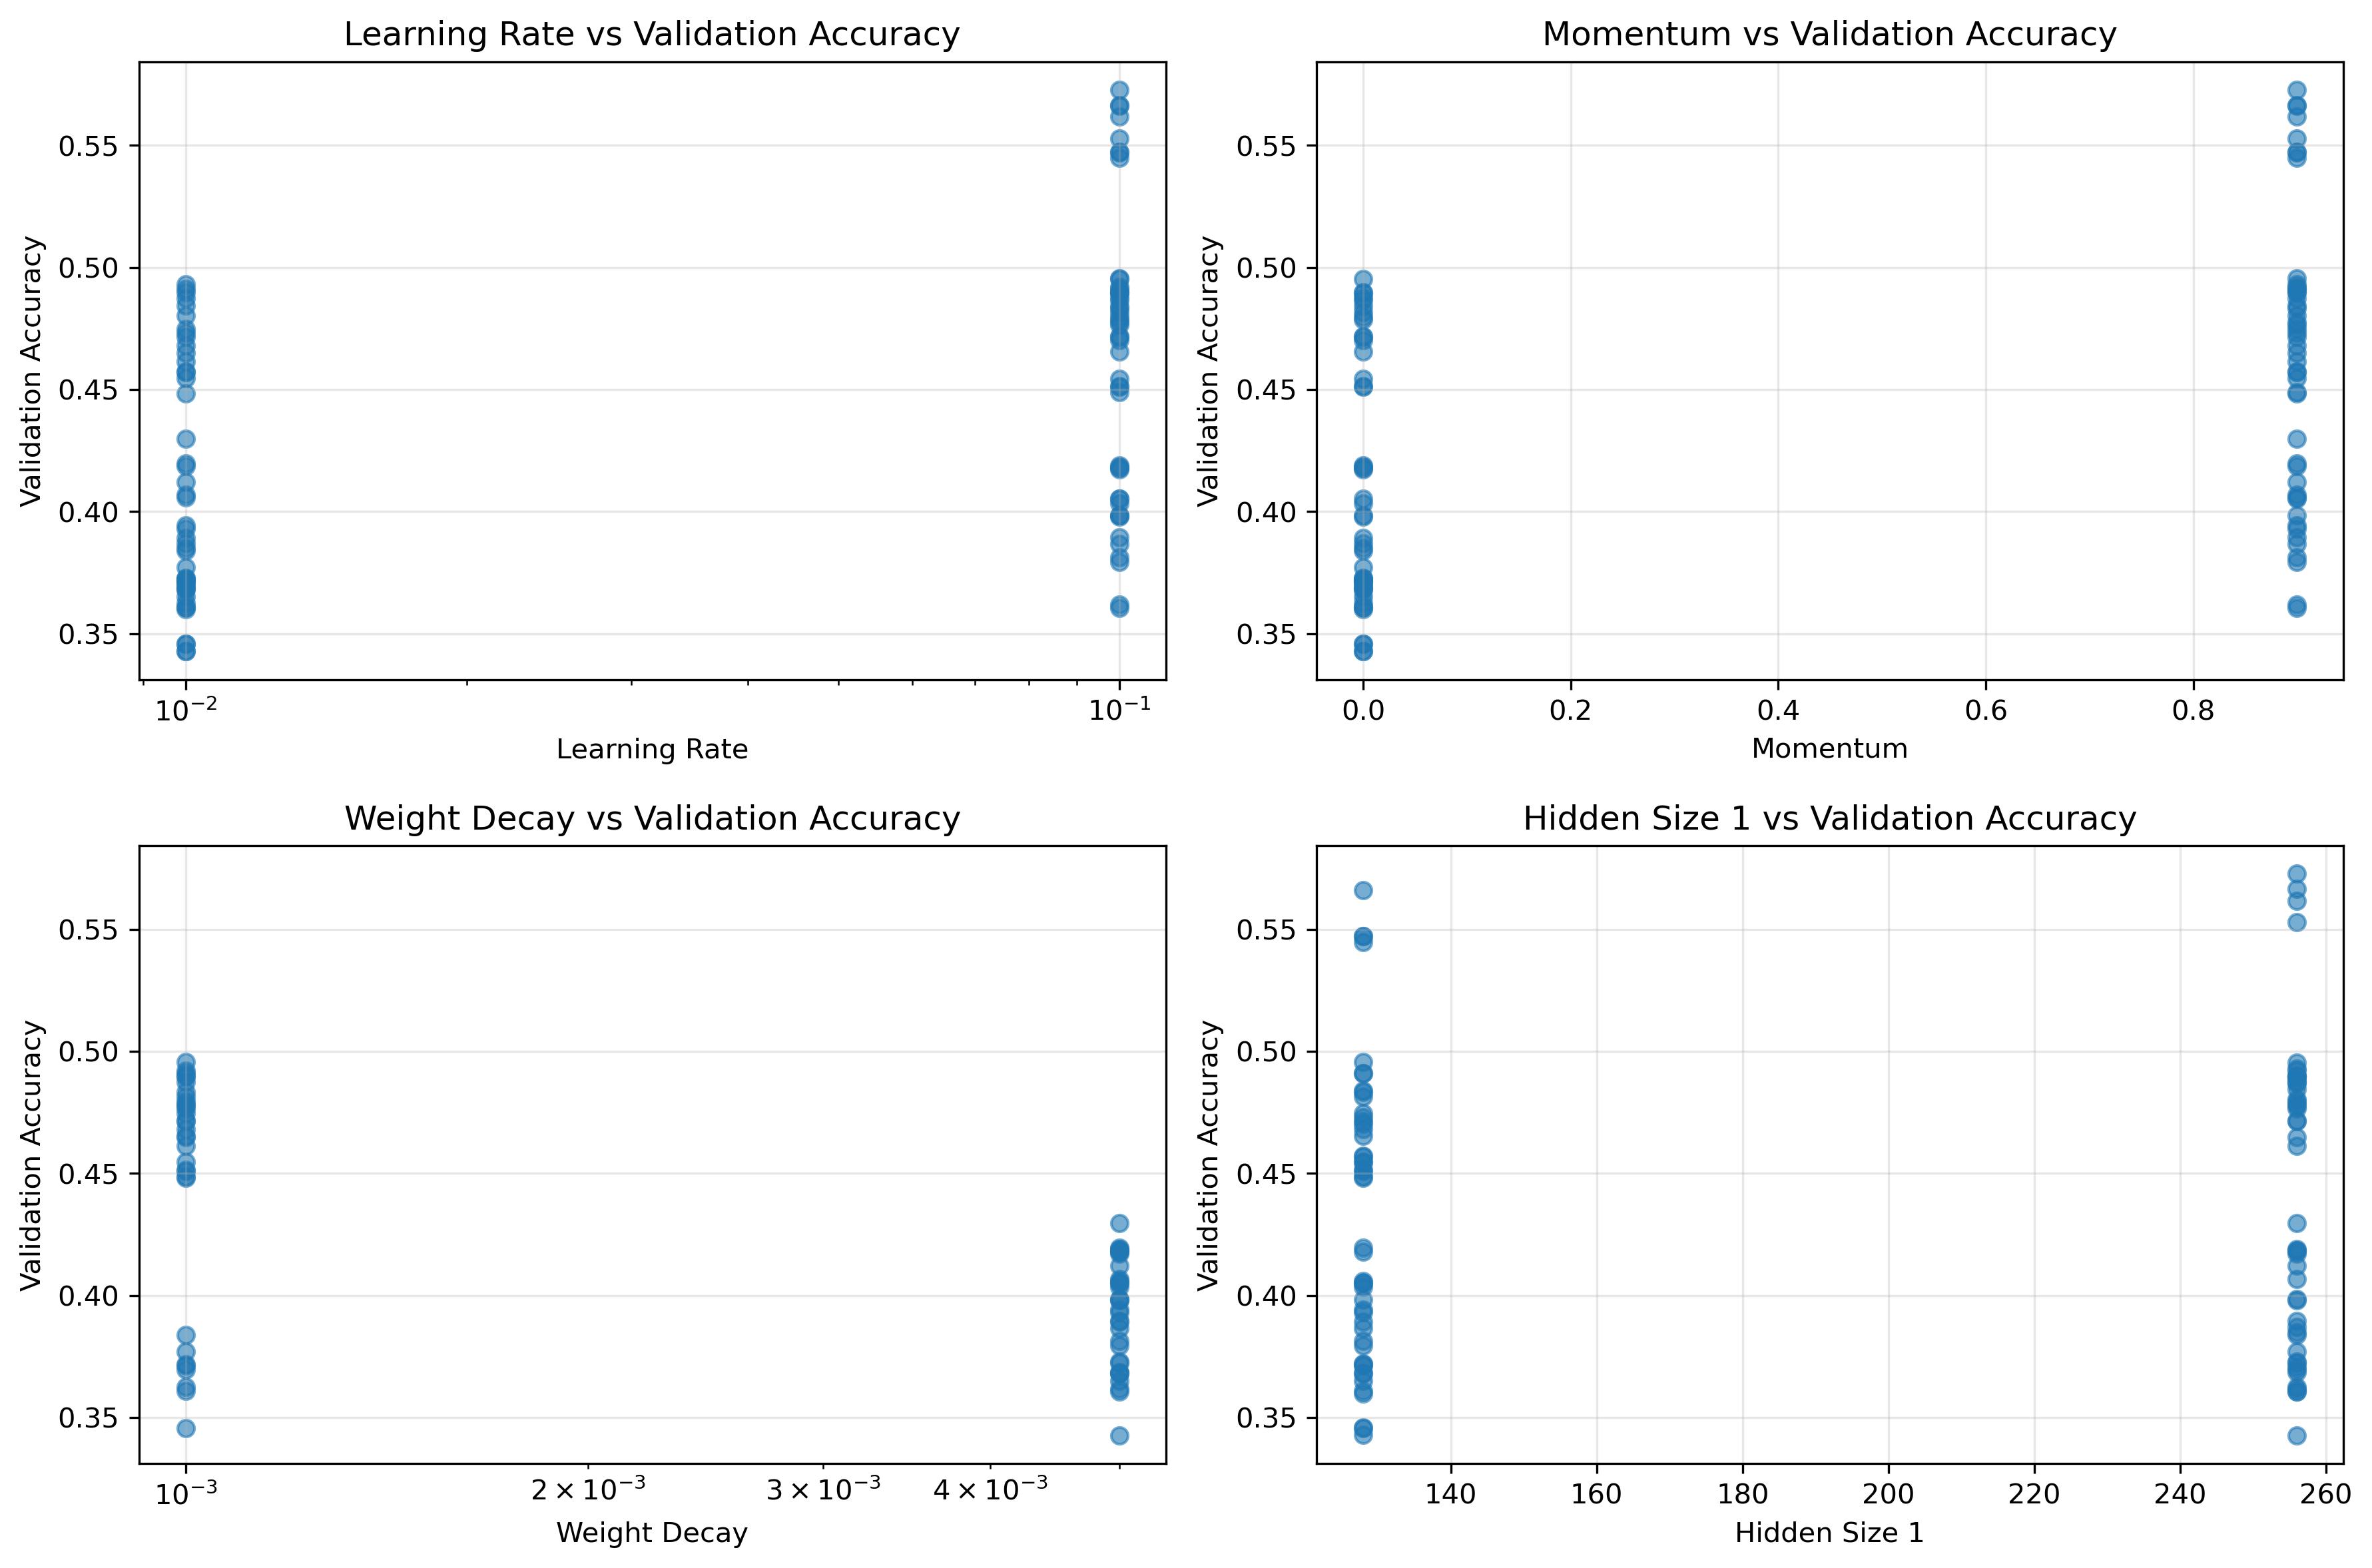
\includegraphics[width=0.9\linewidth]{../search_results/visualizations/hyperparam_importance.png}
    \captionsetup{font={small,bf}}  % 小号加粗
    \caption{超参数重要性分析}
    \label{fig:hyperparam_importance}
\end{figure}
从图中可以看出，学习率和动量对模型性能的影响较大，而权重衰减的影响相对较小。
\subsubsection{准确率分布}
所有超参数配置的准确率分布如图~\ref{fig:accuracy_distribution}所示：
\begin{figure}[!htb]
    \centering
    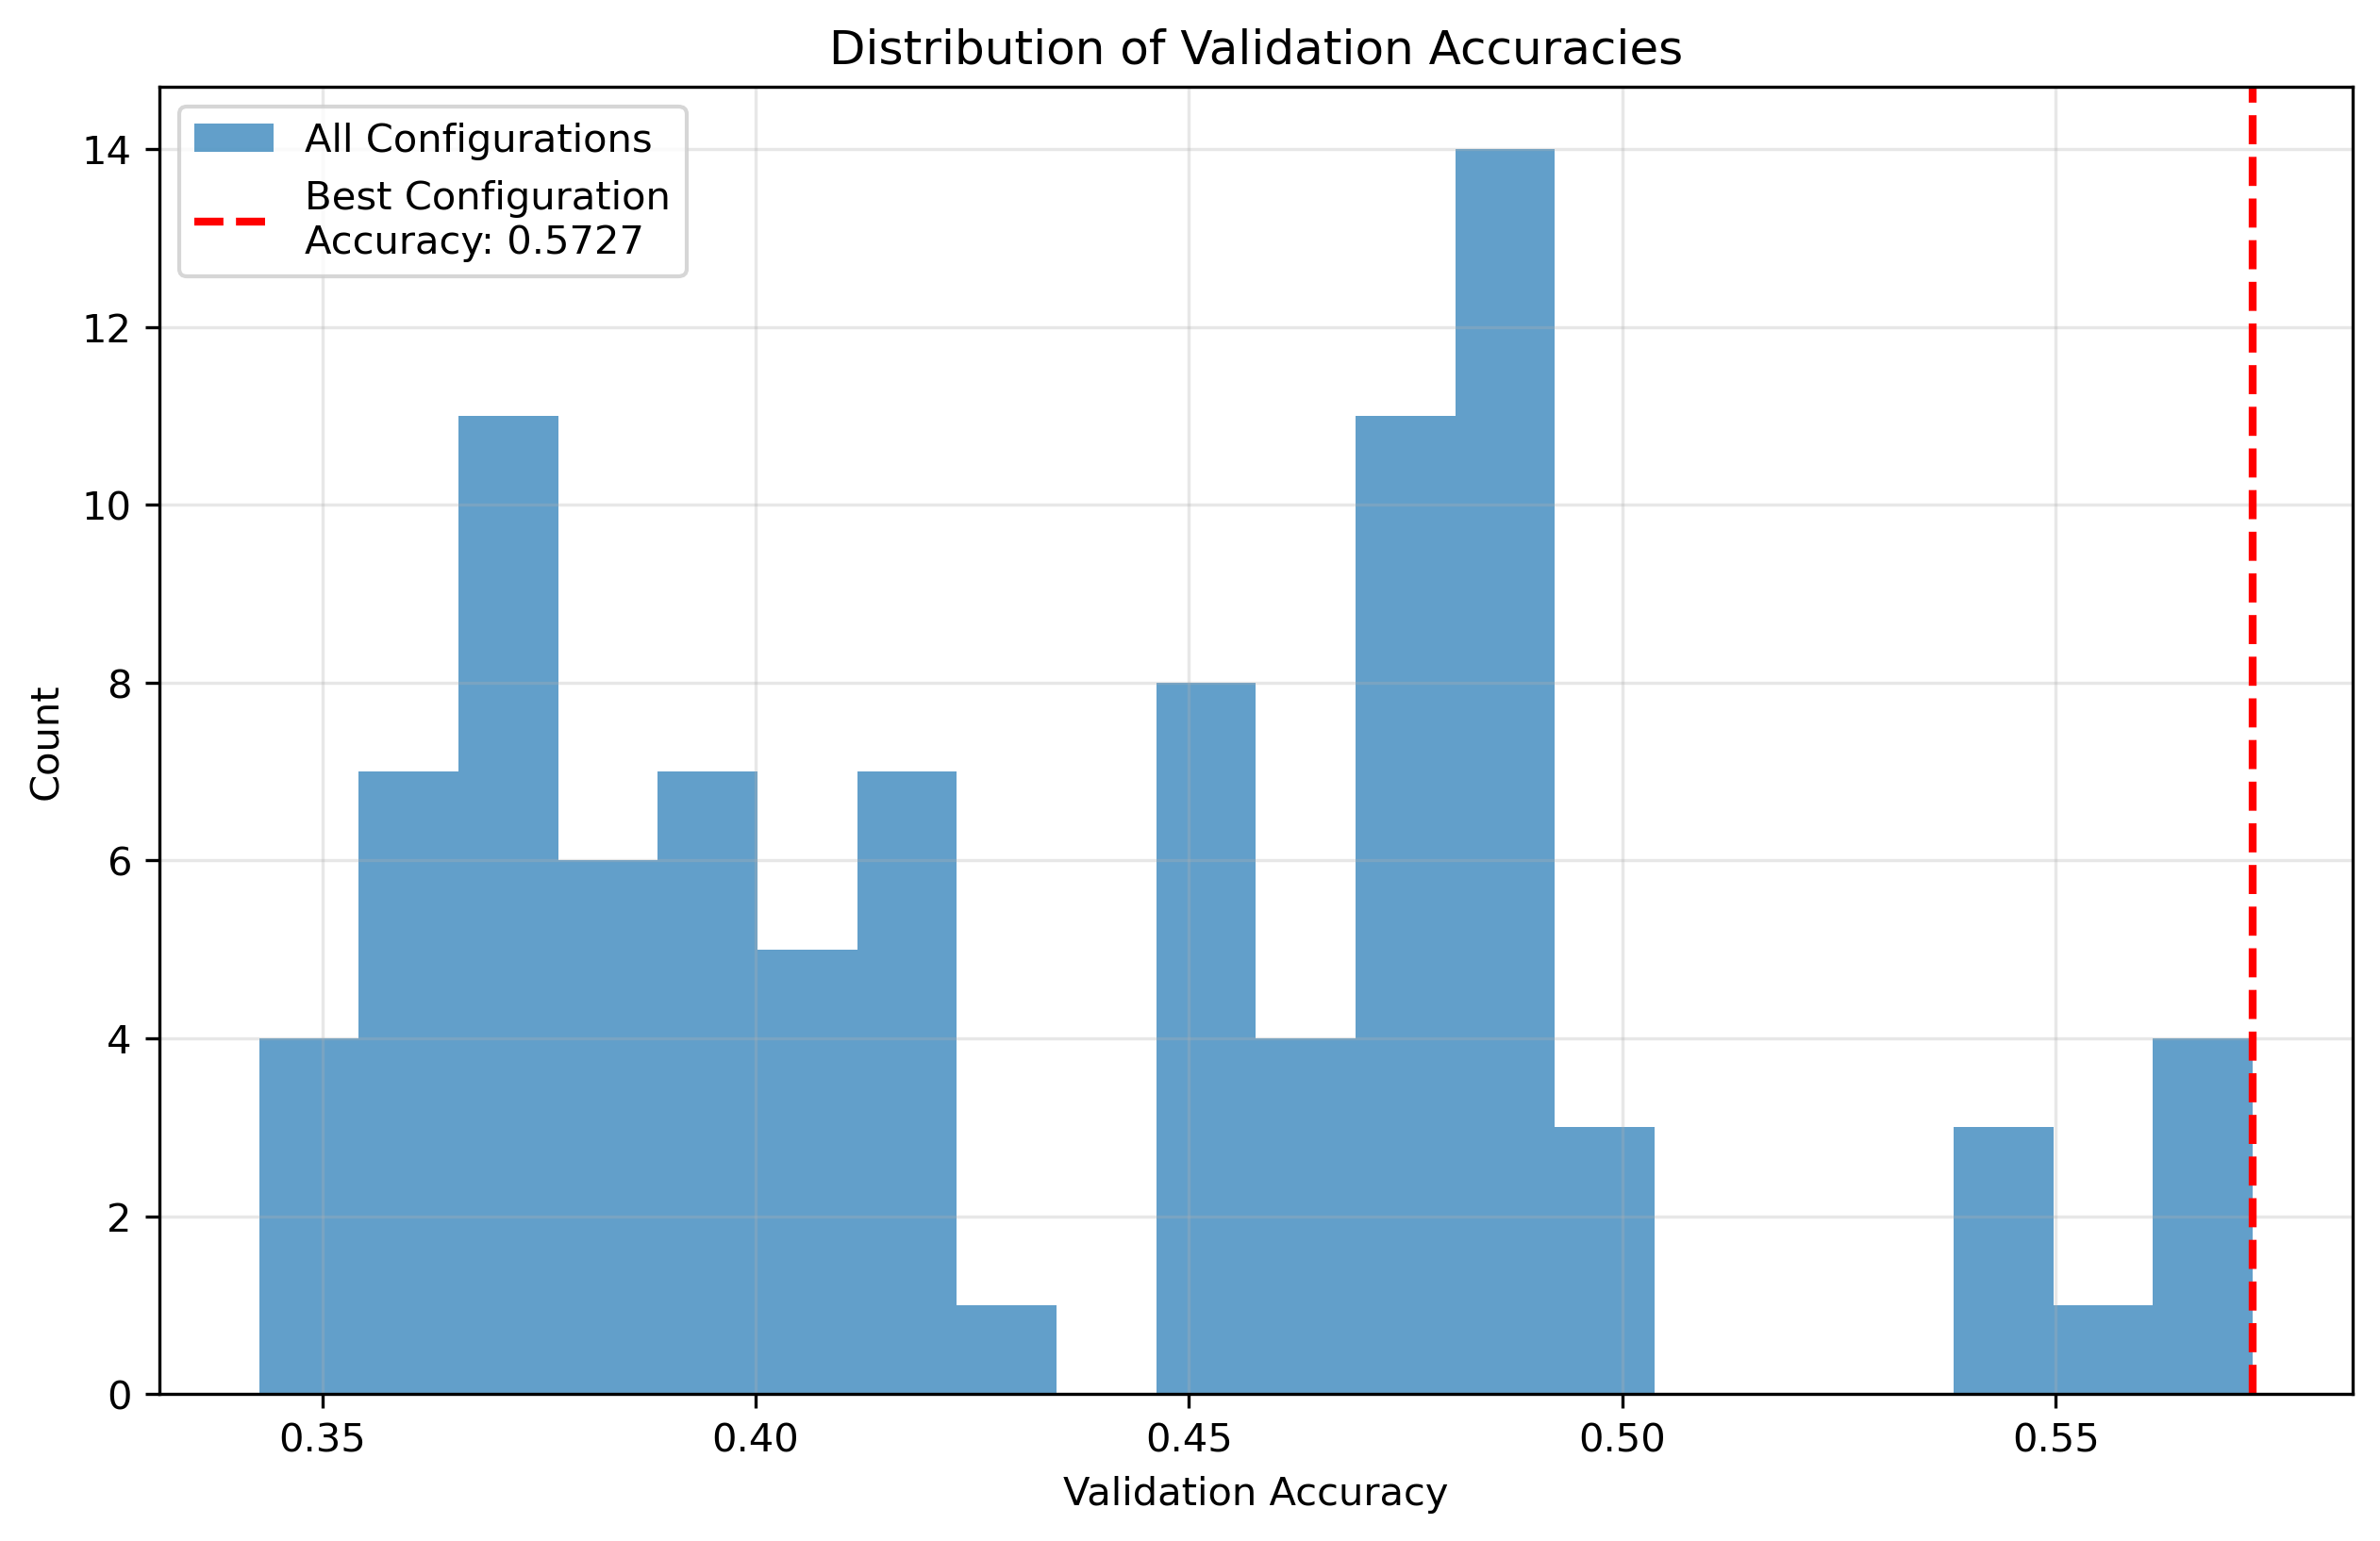
\includegraphics[width=0.7\linewidth]{../search_results/visualizations/accuracy_distribution.png}
    \captionsetup{font={small,bf}}  % 小号加粗
    \caption{验证准确率分布}
    \label{fig:accuracy_distribution}
\end{figure}
\subsection{模型性能评估}
\subsubsection{测试集准确率}
最佳模型在测试集上的准确率为：\textbf{59.83\%}
\subsubsection{混淆矩阵}
模型在测试集上的混淆矩阵如图~\ref{fig:confusion_matrix}所示：
\begin{figure}[!htb]
    \centering
    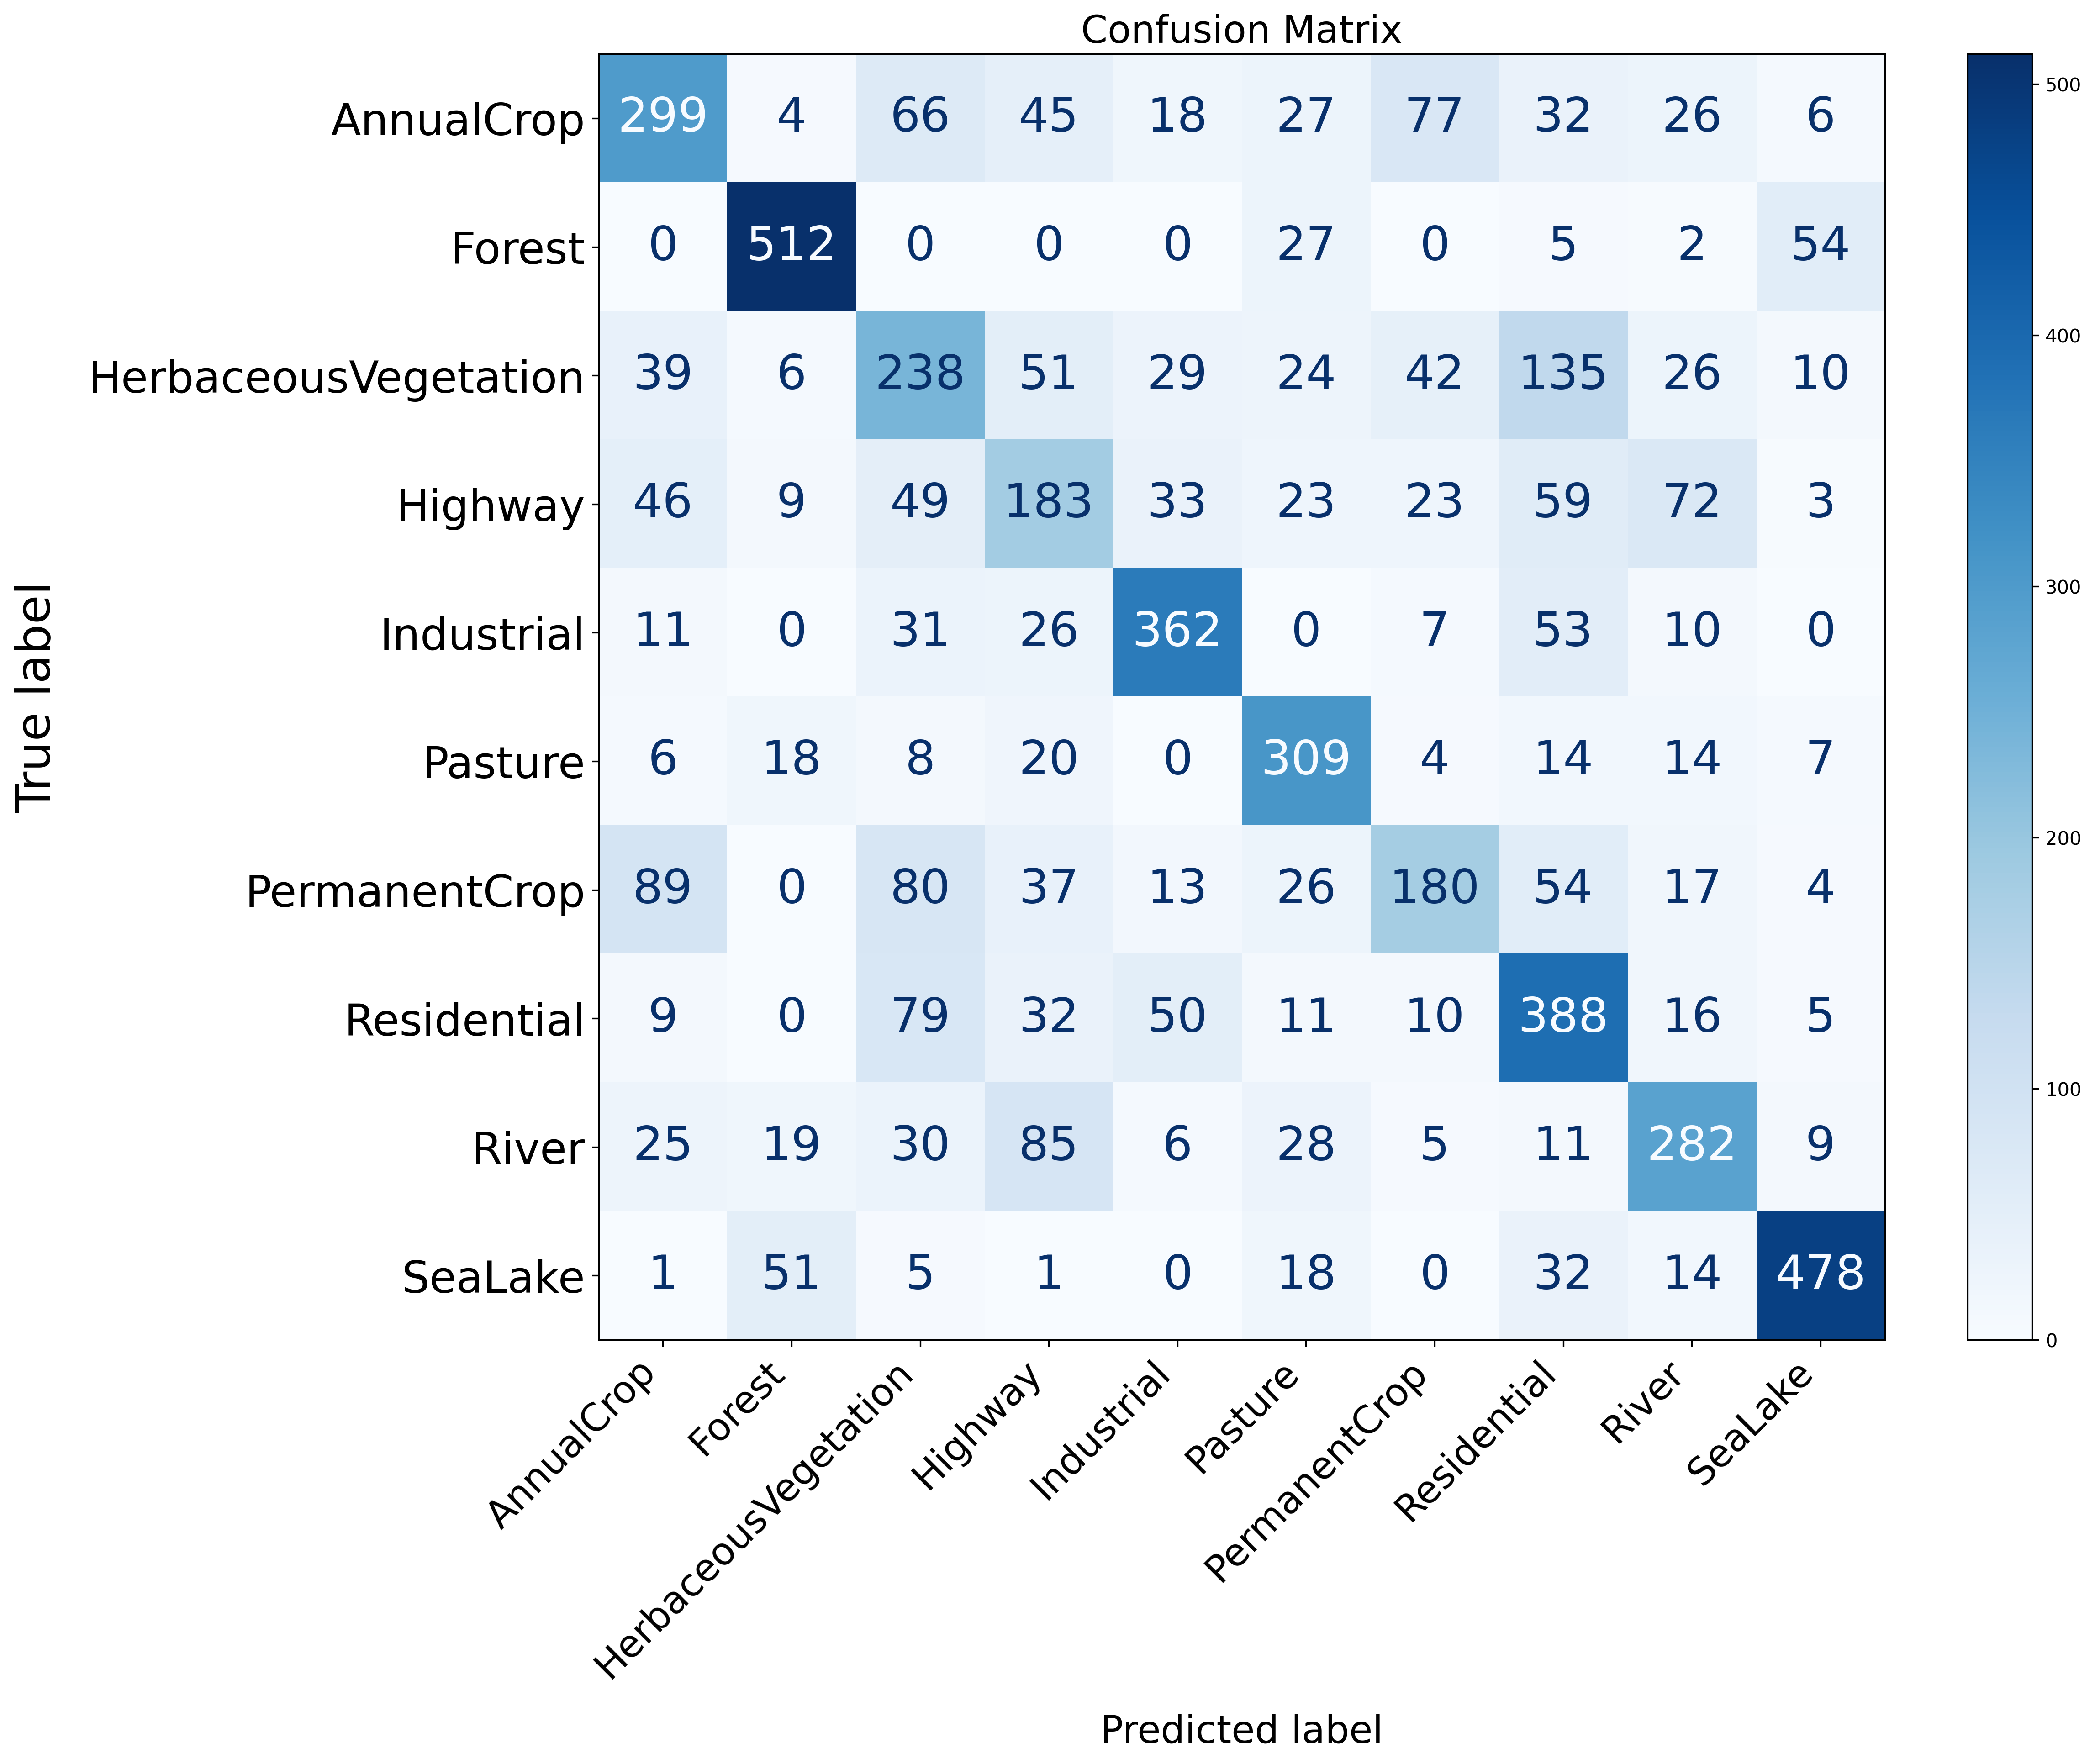
\includegraphics[width=0.7\linewidth]{../results/confusion_matrix.png}
    \captionsetup{font={small,bf}}  % 小号加粗
    \caption{测试集混淆矩阵}
    \label{fig:confusion_matrix}
\end{figure}
从混淆矩阵可以看出，模型在森林、河流等类别上表现较好，而在工业区域和人造区域等类别上容易混淆。
\subsection{训练过程可视化}
\subsubsection{训练历史曲线}
模型的训练历史曲线如图~\ref{fig:training_history}所示：
\begin{figure}[!htb]
    \centering
    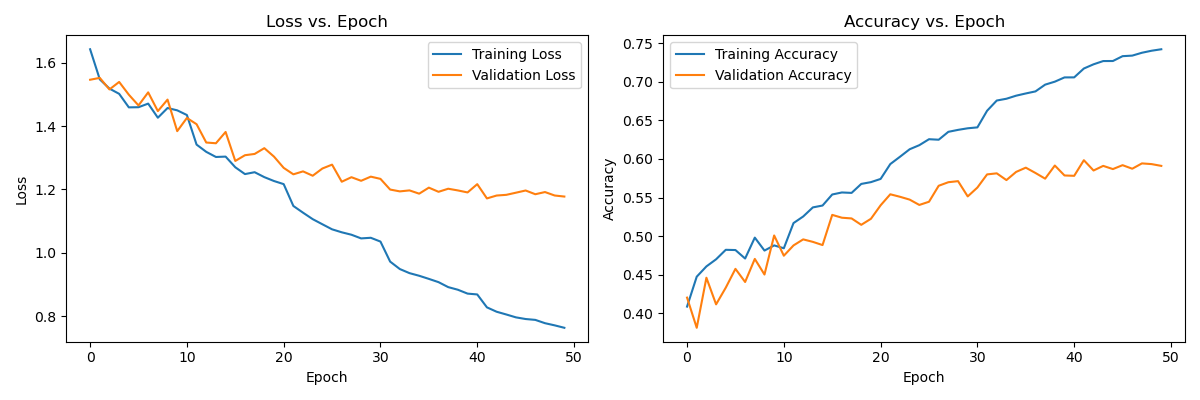
\includegraphics[width=0.9\linewidth]{../models/training_history.png}
    \captionsetup{font={small,bf}}  % 小号加粗
    \caption{训练历史曲线}
    \label{fig:training_history}
\end{figure}
从训练历史曲线可以看出：
\begin{itemize}[topsep=0pt, partopsep=0pt, itemsep=0pt, parsep=0pt]
    \item 训练损失随着训练轮数的增加持续下降，验证损失在前期同步下降，但在第20轮左右趋于稳定，与训练损失的差距逐渐拉大；
    \item 训练准确率随训练轮数持续上升，验证准确率在前期同步提升，在第30轮左右进入平台期，不再明显增长；
    \item 训练集与验证集性能的持续分化，说明模型在训练后期开始过度拟合训练数据中的噪声，存在明显的过拟合风险。
\end{itemize}
\subsubsection{超参数搜索结果}
学习率对模型准确率的影响如图~\ref{fig:learning_rate_vs_accuracy}所示：
\begin{figure}[!htb]
    \centering
    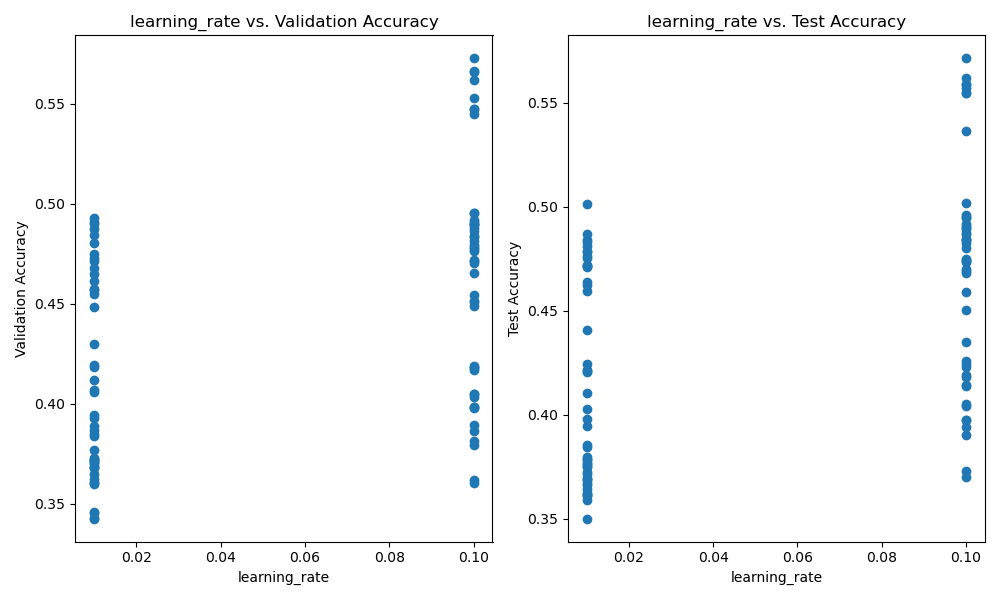
\includegraphics[width=0.7\linewidth]{../search_results/learning_rate_vs_accuracy.png}
    \captionsetup{font={small,bf}}  % 小号加粗
    \caption{学习率对准确率的影响}
    \label{fig:learning_rate_vs_accuracy}
\end{figure}
\subsubsection{隐藏层大小对准确率的影响}
隐藏层大小对模型准确率的影响如图~\ref{fig:hidden_size_vs_accuracy}所示：
\begin{figure}[!htb]
    \centering
    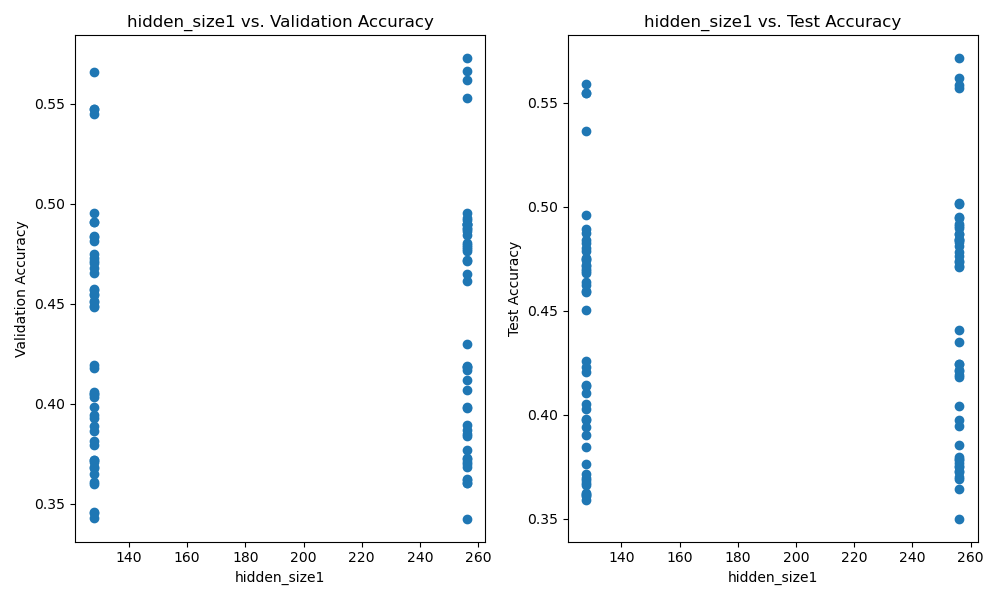
\includegraphics[width=0.7\linewidth]{../search_results/hidden_size1_vs_accuracy.png}
    \captionsetup{font={small,bf}}  % 小号加粗
    \caption{隐藏层1大小对准确率的影响}
    \label{fig:hidden_size_vs_accuracy}
\end{figure}
\subsection{权重可视化}
\subsubsection{第一层权重可视化}
第一层隐藏层权重的可视化结果如图~\ref{fig:first_layer_weights}所示：
\begin{figure}[!htb]
    \centering
    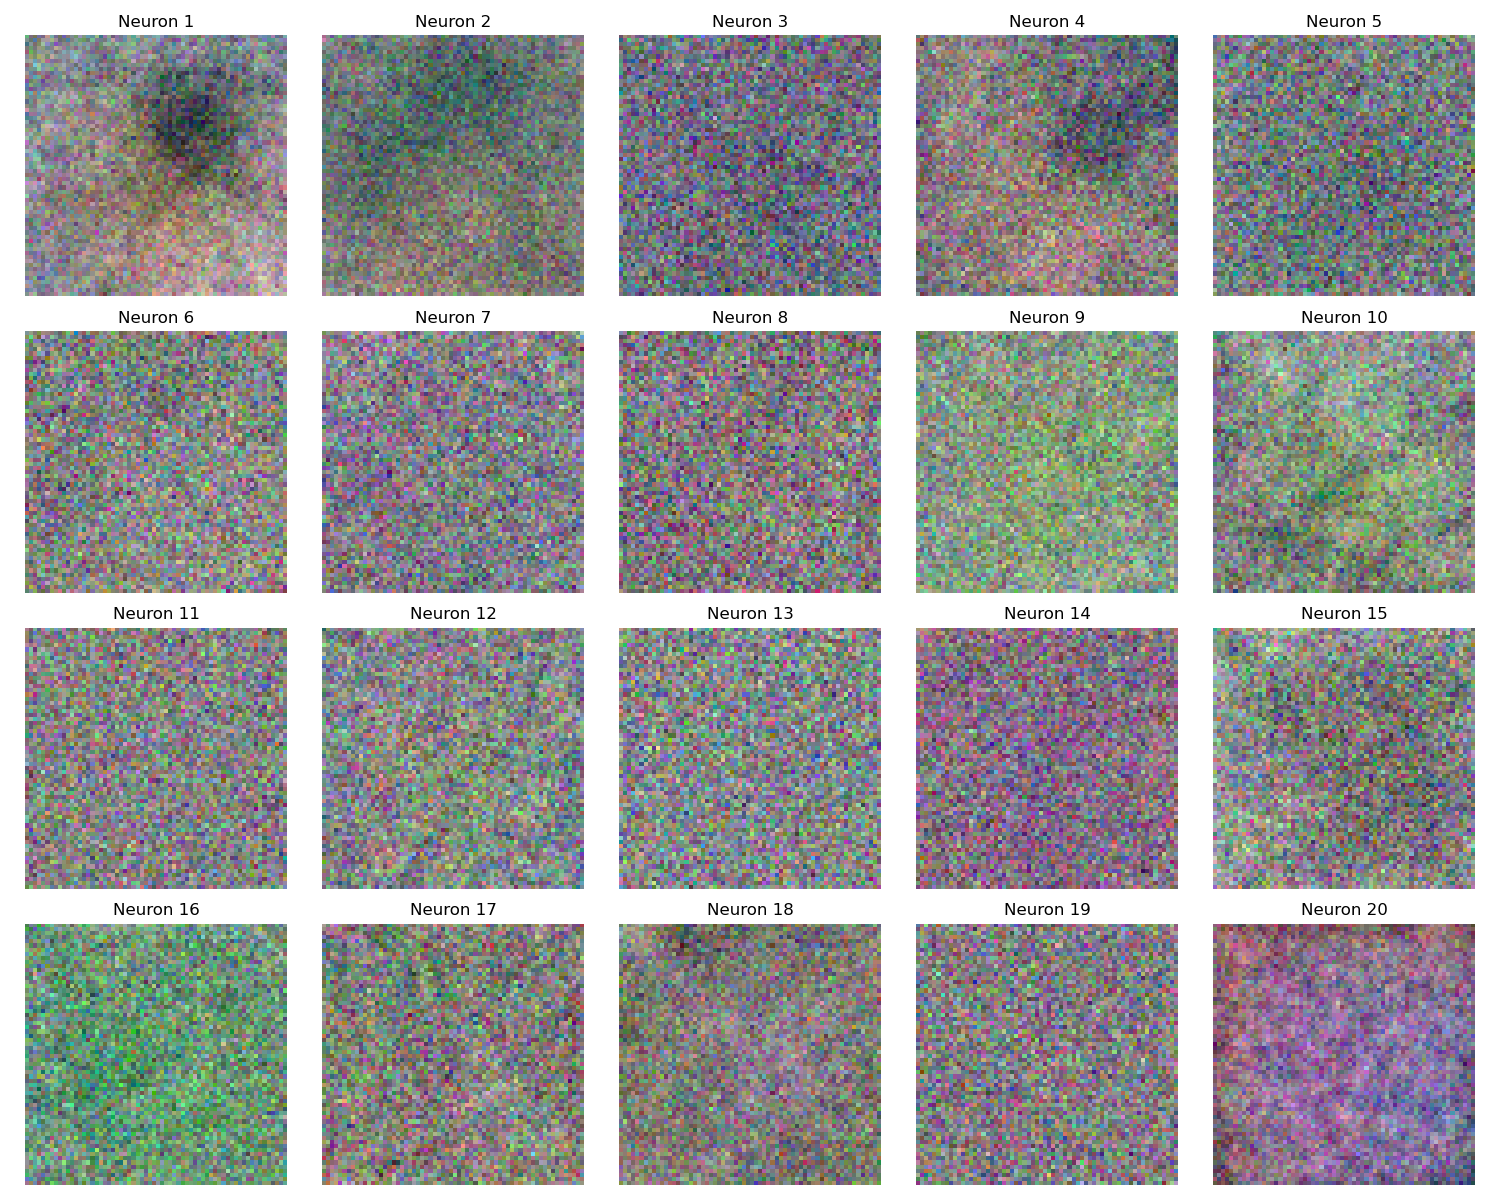
\includegraphics[width=0.7\linewidth]{../results/first_layer_weights.png}
    \captionsetup{font={small,bf}}  % 小号加粗
    \caption{第一层隐藏层权重可视化}
    \label{fig:first_layer_weights}
\end{figure}
从第一层隐藏层权重的可视化结果可以看出，部分神经元已学习到边缘、纹理和颜色等基础视觉特征，而部分神经元的权重仍表现为随机噪声模式，表明其特征学习尚未充分或未被有效激活。

\subsection{错误分析}
\subsubsection{错误分类样本}
错误分类的样本如图~\ref{fig:misclassified_samples}所示：
\begin{figure}[!htb]
    \centering
    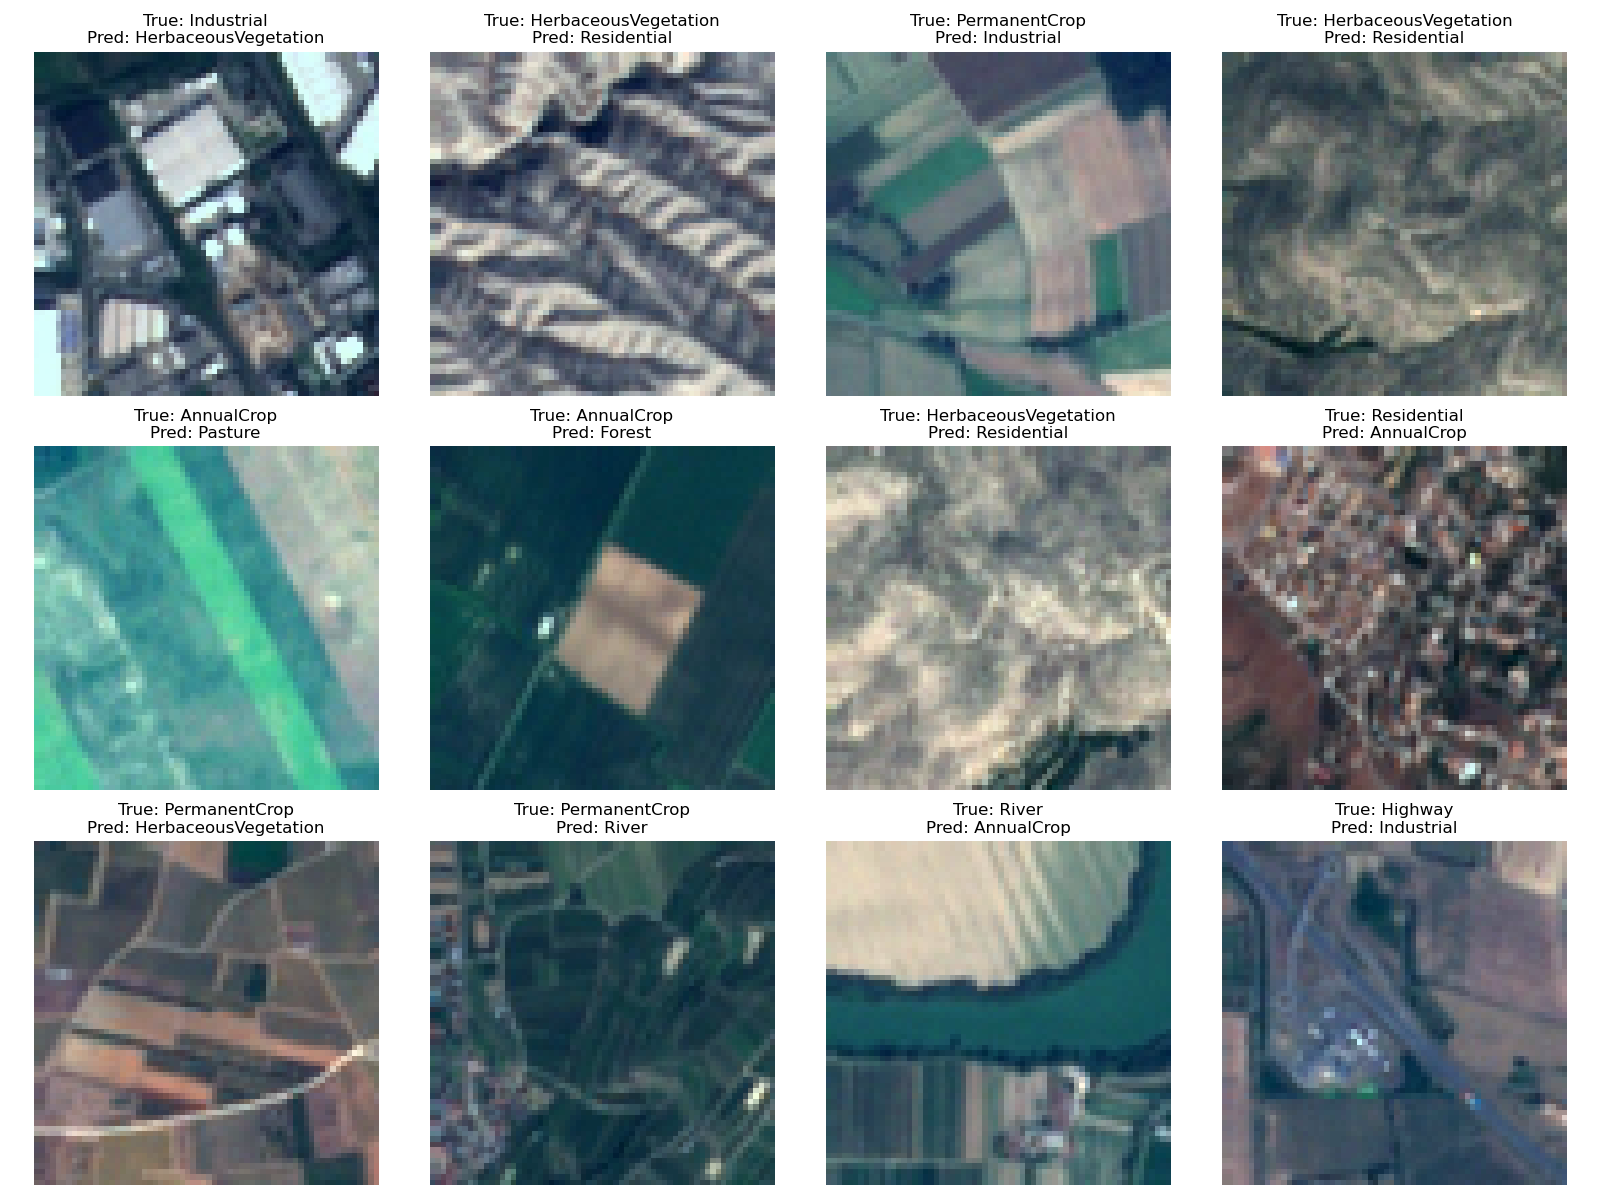
\includegraphics[width=0.7\linewidth]{../results/misclassified_samples.png}
    \captionsetup{font={small,bf}}  % 小号加粗
    \caption{错误分类样本}
    \label{fig:misclassified_samples}
\end{figure}
错误分类的主要原因包括：
\begin{itemize}[topsep=0pt, partopsep=0pt, itemsep=0pt, parsep=0pt]
    \item 植被类地物间（草本植被、牧场、森林、永久/一年生作物）色调、纹理重叠，易互相误判（如图9.1.2、图9.2.1、图9.2.2、图9.3.1）；
    \item 建成区（工业区、居民区）与植被类地物特征混淆（如图9.1.1、图9.1.4、图9.2.3）；
    \item 线性/块状人工地物（高速公路、工业区）与农田/植被纹理存在重叠（如图9.2.4、图9.3.4）；
    \item 水体与农田的边界、色调特征存在混淆（如图9.3.2、图9.3.3）。
    \item 图像分辨率较低，地物细节特征不足，难以区分类间差异。
    \item 光照、拍摄角度等环境因素，导致同类地物的光谱/纹理特征出现较大差异。
\end{itemize}
\subsection{模型保存与访问}

本文训练的最佳模型已上传至Google Drive，可通过以下链接访问：
\begin{center}
\url{https://drive.google.com/file/d/1yvQ8wSRVj85qkrUZv_r169LcEF4ZwK3S/view?usp=sharing}
\end{center}

完整项目代码已上传至GitHub，可通过以下链接访问：
\begin{center}
\url{https://github.com/Fanxiy/Network_byhand}
\end{center}
\section{总结与展望}
\subsection{实验总结}
本文成功实现了一个从零开始构建的三层神经网络分类器，用于EuroSAT-RGB遥感图像分类任务。主要完成了以下工作：
\begin{itemize}[topsep=0pt, partopsep=0pt, itemsep=0pt, parsep=0pt]
    \item 自主实现了自动微分与反向传播，不依赖任何深度学习框架；
    \item 实现了数据加载与预处理、模型定义、训练循环、测试评估、超参数查找五个模块；
    \item 支持自定义隐藏层大小、激活函数切换、学习率衰减和L2正则化；
    \item 进行了超参数搜索，优化了模型性能；
    \item 可视化了训练过程、模型参数和错误分析。
\end{itemize}
实验结果表明，该模型在 EuroSAT 测试集上实现了 59.83\% 的分类准确率。对于仅三层的全连接网络而言，这一结果已达到较为理想的性能表现。
\subsection{技术挑战与解决方案}
在实现过程中，遇到了以下技术挑战：
\begin{itemize}[topsep=0pt, partopsep=0pt, itemsep=0pt, parsep=0pt]
    \item 自动微分与反向传播的实现：通过手动推导梯度公式，实现了各层的反向传播；
    \item 超参数优化：通过网格搜索和随机搜索，找到了最佳的超参数组合；
    \item 模型过拟合：通过L2正则化和学习率衰减，缓解了过拟合问题。
\end{itemize}
\subsection{未来工作展望}
未来工作可以从以下几个方面进行改进：
\begin{itemize}[topsep=0pt, partopsep=0pt, itemsep=0pt, parsep=0pt]
    \item 模型架构优化：尝试使用卷积神经网络（CNN）处理图像数据，提高特征提取能力；
    \item 数据增强：通过旋转、缩放、翻转等数据增强技术，提高模型的泛化能力；
    \item 集成学习：通过集成多个模型，进一步提高分类性能；
    \item 迁移学习：利用预训练模型，提高模型的学习效率和性能。
\end{itemize}



% If you need an appendix, uncomment the following three lines:
% \newpage

\end{document}
% \appendix
% \section*{附录}
